\section{Project management}

\subsection{Preventive planning}
First of all, I developed a Gantt chart (see appendix \ref{appendix:gantt}) to plan the different tasks to be done for the realization of the project, from the project design to the production. To plan the different tasks, I was inspired by the notion of \textit{sprints} of the Agile Scrum method \cite{scrum}. A sprint, as used in this project management, is a one-week application development phase. At the end of a sprint, the functionalities developed during the week must be completed, tested and ready to be available in production.

\begin{figure}
  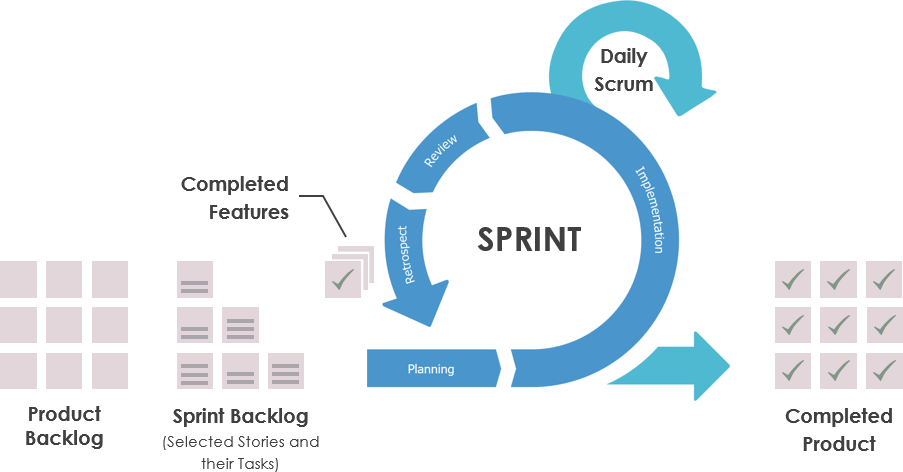
\includegraphics[width=.7\linewidth]{content/imgs/scrum_sprint.png}
  \caption{Scrum sprint}
\end{figure}

Out of the 12 weeks of the internship, 7 weeks were devoted to the development of the application. So, at the beginning of the project, I defined the functionalities of each of the 7 sprints corresponding to the 7 weeks. The first weeks were devoted to discover the topic, do somes researches, drafting specifications and designing the architecture of the application. The last two weeks have been reserved for the final deployment of the application on the \textit{Play Store} and this report.



\subsection{Version management (git)}

I chose to use the version management system \textit{Git} with the hosting service \textit{Github} to give my referent teacher and placement supervisor quick and complete access to the work done on the application.

\textit{Github} also allowed me to create project backups, called \textit{release}, to download the source code of the major versions of the application with the installation file for Android devices. The \textit{release} are also publish with the description of what has changed since the last version (see Appendix \ref{appendix:release}, an example of the last \textit{release} of the project).











% eof
